% Options for packages loaded elsewhere
\PassOptionsToPackage{unicode}{hyperref}
\PassOptionsToPackage{hyphens}{url}
\PassOptionsToPackage{dvipsnames,svgnames,x11names}{xcolor}
%
\documentclass[
  11pt,
]{article}

\usepackage{amsmath,amssymb}
\usepackage{iftex}
\ifPDFTeX
  \usepackage[T1]{fontenc}
  \usepackage[utf8]{inputenc}
  \usepackage{textcomp} % provide euro and other symbols
\else % if luatex or xetex
  \usepackage{unicode-math}
  \defaultfontfeatures{Scale=MatchLowercase}
  \defaultfontfeatures[\rmfamily]{Ligatures=TeX,Scale=1}
\fi
\usepackage{lmodern}
\ifPDFTeX\else  
    % xetex/luatex font selection
\fi
% Use upquote if available, for straight quotes in verbatim environments
\IfFileExists{upquote.sty}{\usepackage{upquote}}{}
\IfFileExists{microtype.sty}{% use microtype if available
  \usepackage[]{microtype}
  \UseMicrotypeSet[protrusion]{basicmath} % disable protrusion for tt fonts
}{}
\makeatletter
\@ifundefined{KOMAClassName}{% if non-KOMA class
  \IfFileExists{parskip.sty}{%
    \usepackage{parskip}
  }{% else
    \setlength{\parindent}{0pt}
    \setlength{\parskip}{6pt plus 2pt minus 1pt}}
}{% if KOMA class
  \KOMAoptions{parskip=half}}
\makeatother
\usepackage{xcolor}
\usepackage[margin=1in]{geometry}
\setlength{\emergencystretch}{3em} % prevent overfull lines
\setcounter{secnumdepth}{5}
% Make \paragraph and \subparagraph free-standing
\ifx\paragraph\undefined\else
  \let\oldparagraph\paragraph
  \renewcommand{\paragraph}[1]{\oldparagraph{#1}\mbox{}}
\fi
\ifx\subparagraph\undefined\else
  \let\oldsubparagraph\subparagraph
  \renewcommand{\subparagraph}[1]{\oldsubparagraph{#1}\mbox{}}
\fi

\usepackage{color}
\usepackage{fancyvrb}
\newcommand{\VerbBar}{|}
\newcommand{\VERB}{\Verb[commandchars=\\\{\}]}
\DefineVerbatimEnvironment{Highlighting}{Verbatim}{commandchars=\\\{\}}
% Add ',fontsize=\small' for more characters per line
\usepackage{framed}
\definecolor{shadecolor}{RGB}{241,243,245}
\newenvironment{Shaded}{\begin{snugshade}}{\end{snugshade}}
\newcommand{\AlertTok}[1]{\textcolor[rgb]{0.68,0.00,0.00}{#1}}
\newcommand{\AnnotationTok}[1]{\textcolor[rgb]{0.37,0.37,0.37}{#1}}
\newcommand{\AttributeTok}[1]{\textcolor[rgb]{0.40,0.45,0.13}{#1}}
\newcommand{\BaseNTok}[1]{\textcolor[rgb]{0.68,0.00,0.00}{#1}}
\newcommand{\BuiltInTok}[1]{\textcolor[rgb]{0.00,0.23,0.31}{#1}}
\newcommand{\CharTok}[1]{\textcolor[rgb]{0.13,0.47,0.30}{#1}}
\newcommand{\CommentTok}[1]{\textcolor[rgb]{0.37,0.37,0.37}{#1}}
\newcommand{\CommentVarTok}[1]{\textcolor[rgb]{0.37,0.37,0.37}{\textit{#1}}}
\newcommand{\ConstantTok}[1]{\textcolor[rgb]{0.56,0.35,0.01}{#1}}
\newcommand{\ControlFlowTok}[1]{\textcolor[rgb]{0.00,0.23,0.31}{#1}}
\newcommand{\DataTypeTok}[1]{\textcolor[rgb]{0.68,0.00,0.00}{#1}}
\newcommand{\DecValTok}[1]{\textcolor[rgb]{0.68,0.00,0.00}{#1}}
\newcommand{\DocumentationTok}[1]{\textcolor[rgb]{0.37,0.37,0.37}{\textit{#1}}}
\newcommand{\ErrorTok}[1]{\textcolor[rgb]{0.68,0.00,0.00}{#1}}
\newcommand{\ExtensionTok}[1]{\textcolor[rgb]{0.00,0.23,0.31}{#1}}
\newcommand{\FloatTok}[1]{\textcolor[rgb]{0.68,0.00,0.00}{#1}}
\newcommand{\FunctionTok}[1]{\textcolor[rgb]{0.28,0.35,0.67}{#1}}
\newcommand{\ImportTok}[1]{\textcolor[rgb]{0.00,0.46,0.62}{#1}}
\newcommand{\InformationTok}[1]{\textcolor[rgb]{0.37,0.37,0.37}{#1}}
\newcommand{\KeywordTok}[1]{\textcolor[rgb]{0.00,0.23,0.31}{#1}}
\newcommand{\NormalTok}[1]{\textcolor[rgb]{0.00,0.23,0.31}{#1}}
\newcommand{\OperatorTok}[1]{\textcolor[rgb]{0.37,0.37,0.37}{#1}}
\newcommand{\OtherTok}[1]{\textcolor[rgb]{0.00,0.23,0.31}{#1}}
\newcommand{\PreprocessorTok}[1]{\textcolor[rgb]{0.68,0.00,0.00}{#1}}
\newcommand{\RegionMarkerTok}[1]{\textcolor[rgb]{0.00,0.23,0.31}{#1}}
\newcommand{\SpecialCharTok}[1]{\textcolor[rgb]{0.37,0.37,0.37}{#1}}
\newcommand{\SpecialStringTok}[1]{\textcolor[rgb]{0.13,0.47,0.30}{#1}}
\newcommand{\StringTok}[1]{\textcolor[rgb]{0.13,0.47,0.30}{#1}}
\newcommand{\VariableTok}[1]{\textcolor[rgb]{0.07,0.07,0.07}{#1}}
\newcommand{\VerbatimStringTok}[1]{\textcolor[rgb]{0.13,0.47,0.30}{#1}}
\newcommand{\WarningTok}[1]{\textcolor[rgb]{0.37,0.37,0.37}{\textit{#1}}}

\providecommand{\tightlist}{%
  \setlength{\itemsep}{0pt}\setlength{\parskip}{0pt}}\usepackage{longtable,booktabs,array}
\usepackage{calc} % for calculating minipage widths
% Correct order of tables after \paragraph or \subparagraph
\usepackage{etoolbox}
\makeatletter
\patchcmd\longtable{\par}{\if@noskipsec\mbox{}\fi\par}{}{}
\makeatother
% Allow footnotes in longtable head/foot
\IfFileExists{footnotehyper.sty}{\usepackage{footnotehyper}}{\usepackage{footnote}}
\makesavenoteenv{longtable}
\usepackage{graphicx}
\makeatletter
\def\maxwidth{\ifdim\Gin@nat@width>\linewidth\linewidth\else\Gin@nat@width\fi}
\def\maxheight{\ifdim\Gin@nat@height>\textheight\textheight\else\Gin@nat@height\fi}
\makeatother
% Scale images if necessary, so that they will not overflow the page
% margins by default, and it is still possible to overwrite the defaults
% using explicit options in \includegraphics[width, height, ...]{}
\setkeys{Gin}{width=\maxwidth,height=\maxheight,keepaspectratio}
% Set default figure placement to htbp
\makeatletter
\def\fps@figure{htbp}
\makeatother

\makeatletter
\makeatother
\makeatletter
\makeatother
\makeatletter
\@ifpackageloaded{caption}{}{\usepackage{caption}}
\AtBeginDocument{%
\ifdefined\contentsname
  \renewcommand*\contentsname{Table of contents}
\else
  \newcommand\contentsname{Table of contents}
\fi
\ifdefined\listfigurename
  \renewcommand*\listfigurename{List of Figures}
\else
  \newcommand\listfigurename{List of Figures}
\fi
\ifdefined\listtablename
  \renewcommand*\listtablename{List of Tables}
\else
  \newcommand\listtablename{List of Tables}
\fi
\ifdefined\figurename
  \renewcommand*\figurename{Figure}
\else
  \newcommand\figurename{Figure}
\fi
\ifdefined\tablename
  \renewcommand*\tablename{Table}
\else
  \newcommand\tablename{Table}
\fi
}
\@ifpackageloaded{float}{}{\usepackage{float}}
\floatstyle{ruled}
\@ifundefined{c@chapter}{\newfloat{codelisting}{h}{lop}}{\newfloat{codelisting}{h}{lop}[chapter]}
\floatname{codelisting}{Listing}
\newcommand*\listoflistings{\listof{codelisting}{List of Listings}}
\makeatother
\makeatletter
\@ifpackageloaded{caption}{}{\usepackage{caption}}
\@ifpackageloaded{subcaption}{}{\usepackage{subcaption}}
\makeatother
\makeatletter
\@ifpackageloaded{tcolorbox}{}{\usepackage[skins,breakable]{tcolorbox}}
\makeatother
\makeatletter
\@ifundefined{shadecolor}{\definecolor{shadecolor}{rgb}{.97, .97, .97}}
\makeatother
\makeatletter
\makeatother
\makeatletter
\makeatother
\ifLuaTeX
  \usepackage{selnolig}  % disable illegal ligatures
\fi
\IfFileExists{bookmark.sty}{\usepackage{bookmark}}{\usepackage{hyperref}}
\IfFileExists{xurl.sty}{\usepackage{xurl}}{} % add URL line breaks if available
\urlstyle{same} % disable monospaced font for URLs
\hypersetup{
  pdftitle={A Project for Reproducible Research},
  pdfauthor={Adnan Sevinc (437971); Le Nhat Tung (426246); Temmuz Burak Yavuzer (444130)},
  colorlinks=true,
  linkcolor={blue},
  filecolor={Maroon},
  citecolor={Blue},
  urlcolor={Blue},
  pdfcreator={LaTeX via pandoc}}

\title{A Project for Reproducible Research}
\usepackage{etoolbox}
\makeatletter
\providecommand{\subtitle}[1]{% add subtitle to \maketitle
  \apptocmd{\@title}{\par {\large #1 \par}}{}{}
}
\makeatother
\subtitle{PDF and LaTeX}
\author{Adnan Sevinc (437971) \and Le Nhat Tung (426246) \and Temmuz
Burak Yavuzer (444130)}
\date{2023-06-09}

\begin{document}
\maketitle
\ifdefined\Shaded\renewenvironment{Shaded}{\begin{tcolorbox}[boxrule=0pt, interior hidden, borderline west={3pt}{0pt}{shadecolor}, enhanced, frame hidden, breakable, sharp corners]}{\end{tcolorbox}}\fi

\begin{center}\rule{0.5\linewidth}{0.5pt}\end{center}

\hypertarget{introduction}{%
\section{Introduction}\label{introduction}}

The aim of this project is to assess the validity of the published
\href{https://www.sciencedirect.com/science/article/abs/pii/S1364032116000848}{article}
from a prominent publisher. namely, to check whether the published
article is consistent or not.

We decided to employ the reproducible research on the selected article
because of the fact that there are many articles in the literature in
order to investigate the relationship between energy consumption and
energy use and their result is somehow contradictory. The relationship
between energy consumption and carbon dioxide (indicator of
environmental deterioration) observed differently due to either dataset
or/and region. Considering all of the inconsistency it will be a great
experience for us to check its validity.

The dataset of the article obtained from
\href{http://data.worldbank.org/indicator}{World Data Bank Indicator}

The code and report of our project can be accessed from
\href{https://github.com/lenhattung/RRProject_426246_437971_444130.git}{repository}

\begin{center}\rule{0.5\linewidth}{0.5pt}\end{center}

\hypertarget{install-required-packages}{%
\section{Install Required Packages}\label{install-required-packages}}

\begin{Shaded}
\begin{Highlighting}[]
\ControlFlowTok{if}\NormalTok{ (}\SpecialCharTok{!}\FunctionTok{require}\NormalTok{(}\StringTok{"pacman"}\NormalTok{)) }\FunctionTok{install.packages}\NormalTok{(}\StringTok{"pacman"}\NormalTok{)}
\end{Highlighting}
\end{Shaded}

\begin{verbatim}
Loading required package: pacman
\end{verbatim}

\begin{Shaded}
\begin{Highlighting}[]
\NormalTok{pacman}\SpecialCharTok{::}\FunctionTok{p\_load}\NormalTok{(                                }
               \StringTok{"ggplot2"}\NormalTok{,}
               \StringTok{"tidyverse"}\NormalTok{,}
               \StringTok{"dplyr"}\NormalTok{,}
               \StringTok{"wbstats"}\NormalTok{,}
               \StringTok{"gmm"}\NormalTok{,}
               \StringTok{"reticulate"}\NormalTok{,}
               \StringTok{"data.table"}\NormalTok{,}
               \StringTok{"panelvar"}\NormalTok{,}
               \StringTok{"pdynmc"}\NormalTok{,}
               \StringTok{"tidyr"}\NormalTok{,}
               \StringTok{"plm"}\NormalTok{,}
               \StringTok{"pastecs"}\NormalTok{,}
               \StringTok{"stargazer"}\NormalTok{,}
               \StringTok{"scales"}
\NormalTok{)}
\end{Highlighting}
\end{Shaded}

\begin{verbatim}
Installing package into 'C:/Users/Biuro Desktop 3/AppData/Local/R/win-library/4.3'
(as 'lib' is unspecified)
\end{verbatim}

\begin{verbatim}
also installing the dependencies 'colorspace', 'utf8', 'farver', 'labeling', 'munsell', 'RColorBrewer', 'viridisLite', 'fansi', 'pillar', 'pkgconfig', 'gtable', 'isoband', 'scales', 'tibble', 'withr'
\end{verbatim}

\begin{verbatim}
Warning: unable to access index for repository http://www.stats.ox.ac.uk/pub/RWin/bin/windows/contrib/4.3:
  cannot open URL 'http://www.stats.ox.ac.uk/pub/RWin/bin/windows/contrib/4.3/PACKAGES'
\end{verbatim}

\begin{verbatim}
package 'colorspace' successfully unpacked and MD5 sums checked
package 'utf8' successfully unpacked and MD5 sums checked
package 'farver' successfully unpacked and MD5 sums checked
package 'labeling' successfully unpacked and MD5 sums checked
package 'munsell' successfully unpacked and MD5 sums checked
package 'RColorBrewer' successfully unpacked and MD5 sums checked
package 'viridisLite' successfully unpacked and MD5 sums checked
package 'fansi' successfully unpacked and MD5 sums checked
package 'pillar' successfully unpacked and MD5 sums checked
package 'pkgconfig' successfully unpacked and MD5 sums checked
package 'gtable' successfully unpacked and MD5 sums checked
package 'isoband' successfully unpacked and MD5 sums checked
package 'scales' successfully unpacked and MD5 sums checked
package 'tibble' successfully unpacked and MD5 sums checked
package 'withr' successfully unpacked and MD5 sums checked
package 'ggplot2' successfully unpacked and MD5 sums checked

The downloaded binary packages are in
    C:\Users\Biuro Desktop 3\AppData\Local\Temp\Rtmp2LQgCe\downloaded_packages
\end{verbatim}

\begin{verbatim}

ggplot2 installed
\end{verbatim}

\begin{verbatim}
Installing package into 'C:/Users/Biuro Desktop 3/AppData/Local/R/win-library/4.3'
(as 'lib' is unspecified)
\end{verbatim}

\begin{verbatim}
also installing the dependencies 'sys', 'bit', 'ps', 'rematch', 'askpass', 'bit64', 'prettyunits', 'processx', 'backports', 'generics', 'blob', 'DBI', 'tidyselect', 'data.table', 'gargle', 'uuid', 'cellranger', 'curl', 'ids', 'rematch2', 'cpp11', 'openssl', 'timechange', 'systemfonts', 'textshaping', 'clipr', 'crayon', 'vroom', 'tzdb', 'progress', 'callr', 'selectr', 'broom', 'conflicted', 'dbplyr', 'dplyr', 'dtplyr', 'forcats', 'googledrive', 'googlesheets4', 'haven', 'hms', 'httr', 'lubridate', 'modelr', 'purrr', 'ragg', 'readr', 'readxl', 'reprex', 'rstudioapi', 'rvest', 'tidyr', 'xml2'
\end{verbatim}

\begin{verbatim}
Warning: unable to access index for repository http://www.stats.ox.ac.uk/pub/RWin/bin/windows/contrib/4.3:
  cannot open URL 'http://www.stats.ox.ac.uk/pub/RWin/bin/windows/contrib/4.3/PACKAGES'
\end{verbatim}

\begin{verbatim}
package 'sys' successfully unpacked and MD5 sums checked
package 'bit' successfully unpacked and MD5 sums checked
package 'ps' successfully unpacked and MD5 sums checked
package 'rematch' successfully unpacked and MD5 sums checked
package 'askpass' successfully unpacked and MD5 sums checked
package 'bit64' successfully unpacked and MD5 sums checked
package 'prettyunits' successfully unpacked and MD5 sums checked
package 'processx' successfully unpacked and MD5 sums checked
package 'backports' successfully unpacked and MD5 sums checked
package 'generics' successfully unpacked and MD5 sums checked
package 'blob' successfully unpacked and MD5 sums checked
package 'DBI' successfully unpacked and MD5 sums checked
package 'tidyselect' successfully unpacked and MD5 sums checked
package 'data.table' successfully unpacked and MD5 sums checked
package 'gargle' successfully unpacked and MD5 sums checked
package 'uuid' successfully unpacked and MD5 sums checked
package 'cellranger' successfully unpacked and MD5 sums checked
package 'curl' successfully unpacked and MD5 sums checked
package 'ids' successfully unpacked and MD5 sums checked
package 'rematch2' successfully unpacked and MD5 sums checked
package 'cpp11' successfully unpacked and MD5 sums checked
package 'openssl' successfully unpacked and MD5 sums checked
package 'timechange' successfully unpacked and MD5 sums checked
package 'systemfonts' successfully unpacked and MD5 sums checked
package 'textshaping' successfully unpacked and MD5 sums checked
package 'clipr' successfully unpacked and MD5 sums checked
package 'crayon' successfully unpacked and MD5 sums checked
package 'vroom' successfully unpacked and MD5 sums checked
package 'tzdb' successfully unpacked and MD5 sums checked
package 'progress' successfully unpacked and MD5 sums checked
package 'callr' successfully unpacked and MD5 sums checked
package 'selectr' successfully unpacked and MD5 sums checked
package 'broom' successfully unpacked and MD5 sums checked
package 'conflicted' successfully unpacked and MD5 sums checked
package 'dbplyr' successfully unpacked and MD5 sums checked
package 'dplyr' successfully unpacked and MD5 sums checked
package 'dtplyr' successfully unpacked and MD5 sums checked
package 'forcats' successfully unpacked and MD5 sums checked
package 'googledrive' successfully unpacked and MD5 sums checked
package 'googlesheets4' successfully unpacked and MD5 sums checked
package 'haven' successfully unpacked and MD5 sums checked
package 'hms' successfully unpacked and MD5 sums checked
package 'httr' successfully unpacked and MD5 sums checked
package 'lubridate' successfully unpacked and MD5 sums checked
package 'modelr' successfully unpacked and MD5 sums checked
package 'purrr' successfully unpacked and MD5 sums checked
package 'ragg' successfully unpacked and MD5 sums checked
package 'readr' successfully unpacked and MD5 sums checked
package 'readxl' successfully unpacked and MD5 sums checked
package 'reprex' successfully unpacked and MD5 sums checked
package 'rstudioapi' successfully unpacked and MD5 sums checked
package 'rvest' successfully unpacked and MD5 sums checked
package 'tidyr' successfully unpacked and MD5 sums checked
package 'xml2' successfully unpacked and MD5 sums checked
package 'tidyverse' successfully unpacked and MD5 sums checked

The downloaded binary packages are in
    C:\Users\Biuro Desktop 3\AppData\Local\Temp\Rtmp2LQgCe\downloaded_packages
\end{verbatim}

\begin{verbatim}

tidyverse installed
\end{verbatim}

\begin{verbatim}
Installing package into 'C:/Users/Biuro Desktop 3/AppData/Local/R/win-library/4.3'
(as 'lib' is unspecified)
\end{verbatim}

\begin{verbatim}
Warning: unable to access index for repository http://www.stats.ox.ac.uk/pub/RWin/bin/windows/contrib/4.3:
  cannot open URL 'http://www.stats.ox.ac.uk/pub/RWin/bin/windows/contrib/4.3/PACKAGES'
\end{verbatim}

\begin{verbatim}
package 'wbstats' successfully unpacked and MD5 sums checked

The downloaded binary packages are in
    C:\Users\Biuro Desktop 3\AppData\Local\Temp\Rtmp2LQgCe\downloaded_packages
\end{verbatim}

\begin{verbatim}

wbstats installed
Installing package into 'C:/Users/Biuro Desktop 3/AppData/Local/R/win-library/4.3'
(as 'lib' is unspecified)
\end{verbatim}

\begin{verbatim}
also installing the dependencies 'zoo', 'sandwich'
\end{verbatim}

\begin{verbatim}
Warning: unable to access index for repository http://www.stats.ox.ac.uk/pub/RWin/bin/windows/contrib/4.3:
  cannot open URL 'http://www.stats.ox.ac.uk/pub/RWin/bin/windows/contrib/4.3/PACKAGES'
\end{verbatim}

\begin{verbatim}
package 'zoo' successfully unpacked and MD5 sums checked
package 'sandwich' successfully unpacked and MD5 sums checked
package 'gmm' successfully unpacked and MD5 sums checked

The downloaded binary packages are in
    C:\Users\Biuro Desktop 3\AppData\Local\Temp\Rtmp2LQgCe\downloaded_packages
\end{verbatim}

\begin{verbatim}

gmm installed
\end{verbatim}

\begin{verbatim}
Installing package into 'C:/Users/Biuro Desktop 3/AppData/Local/R/win-library/4.3'
(as 'lib' is unspecified)
\end{verbatim}

\begin{verbatim}
also installing the dependencies 'rprojroot', 'Rcpp', 'RcppTOML', 'here', 'png'
\end{verbatim}

\begin{verbatim}
Warning: unable to access index for repository http://www.stats.ox.ac.uk/pub/RWin/bin/windows/contrib/4.3:
  cannot open URL 'http://www.stats.ox.ac.uk/pub/RWin/bin/windows/contrib/4.3/PACKAGES'
\end{verbatim}

\begin{verbatim}
package 'rprojroot' successfully unpacked and MD5 sums checked
package 'Rcpp' successfully unpacked and MD5 sums checked
package 'RcppTOML' successfully unpacked and MD5 sums checked
package 'here' successfully unpacked and MD5 sums checked
package 'png' successfully unpacked and MD5 sums checked
package 'reticulate' successfully unpacked and MD5 sums checked

The downloaded binary packages are in
    C:\Users\Biuro Desktop 3\AppData\Local\Temp\Rtmp2LQgCe\downloaded_packages
\end{verbatim}

\begin{verbatim}

reticulate installed
\end{verbatim}

\begin{verbatim}
Installing package into 'C:/Users/Biuro Desktop 3/AppData/Local/R/win-library/4.3'
(as 'lib' is unspecified)
\end{verbatim}

\begin{verbatim}
also installing the dependencies 'plyr', 'matrixcalc', 'texreg', 'reshape2'
\end{verbatim}

\begin{verbatim}
Warning: unable to access index for repository http://www.stats.ox.ac.uk/pub/RWin/bin/windows/contrib/4.3:
  cannot open URL 'http://www.stats.ox.ac.uk/pub/RWin/bin/windows/contrib/4.3/PACKAGES'
\end{verbatim}

\begin{verbatim}
package 'plyr' successfully unpacked and MD5 sums checked
package 'matrixcalc' successfully unpacked and MD5 sums checked
package 'texreg' successfully unpacked and MD5 sums checked
package 'reshape2' successfully unpacked and MD5 sums checked
package 'panelvar' successfully unpacked and MD5 sums checked

The downloaded binary packages are in
    C:\Users\Biuro Desktop 3\AppData\Local\Temp\Rtmp2LQgCe\downloaded_packages
\end{verbatim}

\begin{verbatim}

panelvar installed
\end{verbatim}

\begin{verbatim}
Installing package into 'C:/Users/Biuro Desktop 3/AppData/Local/R/win-library/4.3'
(as 'lib' is unspecified)
\end{verbatim}

\begin{verbatim}
also installing the dependencies 'numDeriv', 'slam', 'sparsesvd', 'docopt', 'rbibutils', 'optimx', 'qlcMatrix', 'Rdpack'
\end{verbatim}

\begin{verbatim}
Warning: unable to access index for repository http://www.stats.ox.ac.uk/pub/RWin/bin/windows/contrib/4.3:
  cannot open URL 'http://www.stats.ox.ac.uk/pub/RWin/bin/windows/contrib/4.3/PACKAGES'
\end{verbatim}

\begin{verbatim}
package 'numDeriv' successfully unpacked and MD5 sums checked
package 'slam' successfully unpacked and MD5 sums checked
package 'sparsesvd' successfully unpacked and MD5 sums checked
package 'docopt' successfully unpacked and MD5 sums checked
package 'rbibutils' successfully unpacked and MD5 sums checked
package 'optimx' successfully unpacked and MD5 sums checked
package 'qlcMatrix' successfully unpacked and MD5 sums checked
package 'Rdpack' successfully unpacked and MD5 sums checked
package 'pdynmc' successfully unpacked and MD5 sums checked

The downloaded binary packages are in
    C:\Users\Biuro Desktop 3\AppData\Local\Temp\Rtmp2LQgCe\downloaded_packages
\end{verbatim}

\begin{verbatim}

pdynmc installed
\end{verbatim}

\begin{verbatim}
Installing package into 'C:/Users/Biuro Desktop 3/AppData/Local/R/win-library/4.3'
(as 'lib' is unspecified)
\end{verbatim}

\begin{verbatim}
also installing the dependencies 'miscTools', 'bdsmatrix', 'collapse', 'lmtest', 'maxLik', 'Formula'
\end{verbatim}

\begin{verbatim}
Warning: unable to access index for repository http://www.stats.ox.ac.uk/pub/RWin/bin/windows/contrib/4.3:
  cannot open URL 'http://www.stats.ox.ac.uk/pub/RWin/bin/windows/contrib/4.3/PACKAGES'
\end{verbatim}

\begin{verbatim}
package 'miscTools' successfully unpacked and MD5 sums checked
package 'bdsmatrix' successfully unpacked and MD5 sums checked
package 'collapse' successfully unpacked and MD5 sums checked
package 'lmtest' successfully unpacked and MD5 sums checked
package 'maxLik' successfully unpacked and MD5 sums checked
package 'Formula' successfully unpacked and MD5 sums checked
package 'plm' successfully unpacked and MD5 sums checked

The downloaded binary packages are in
    C:\Users\Biuro Desktop 3\AppData\Local\Temp\Rtmp2LQgCe\downloaded_packages
\end{verbatim}

\begin{verbatim}

plm installed
\end{verbatim}

\begin{verbatim}
Installing package into 'C:/Users/Biuro Desktop 3/AppData/Local/R/win-library/4.3'
(as 'lib' is unspecified)
\end{verbatim}

\begin{verbatim}
Warning: unable to access index for repository http://www.stats.ox.ac.uk/pub/RWin/bin/windows/contrib/4.3:
  cannot open URL 'http://www.stats.ox.ac.uk/pub/RWin/bin/windows/contrib/4.3/PACKAGES'
\end{verbatim}

\begin{verbatim}
package 'stargazer' successfully unpacked and MD5 sums checked

The downloaded binary packages are in
    C:\Users\Biuro Desktop 3\AppData\Local\Temp\Rtmp2LQgCe\downloaded_packages
\end{verbatim}

\begin{verbatim}

stargazer installed
\end{verbatim}

\begin{Shaded}
\begin{Highlighting}[]
\FunctionTok{Sys.setlocale}\NormalTok{(}\StringTok{"LC\_TIME"}\NormalTok{, }\StringTok{"English"}\NormalTok{)}
\end{Highlighting}
\end{Shaded}

\begin{verbatim}
[1] "English_United States.1252"
\end{verbatim}

\begin{center}\rule{0.5\linewidth}{0.5pt}\end{center}

\hypertarget{dataset}{%
\section{Dataset}\label{dataset}}

Following variables used during modeling process for the time period
spanning from 1990 to 2012.

\begin{longtable}[]{@{}ll@{}}
\toprule\noalign{}
Variables & Abbreviation \\
\midrule\noalign{}
\endhead
\bottomrule\noalign{}
\endlastfoot
CO2 emissions (metric tons per capita) & C \\
Energy use (kg of oil equivalent per capita) & E \\
GDP per capita (constant 2015 US\$) & Y \\
Urban population (\% of total population) & URB \\
Trade (\% of GDP) & TR \\
\end{longtable}

\begin{center}\rule{0.5\linewidth}{0.5pt}\end{center}

\hypertarget{import-dataset}{%
\section{Import Dataset}\label{import-dataset}}

We imported dataset directly from WDI using \textbf{wbstats} packages.

\begin{Shaded}
\begin{Highlighting}[]
\NormalTok{my\_indicators }\OtherTok{\textless{}{-}} \FunctionTok{c}\NormalTok{(                         }
  \AttributeTok{C =} \StringTok{"EN.ATM.CO2E.PC"}\NormalTok{,  }
  \AttributeTok{E =}\StringTok{"EG.USE.PCAP.KG.OE"}\NormalTok{,  }
  \AttributeTok{Y =} \StringTok{"NY.GDP.PCAP.KD"}\NormalTok{, }
  \AttributeTok{URB =} \StringTok{"SP.URB.TOTL.IN.ZS"}\NormalTok{, }
  \AttributeTok{TR =} \StringTok{"NE.TRD.GNFS.ZS"} 
\NormalTok{)}

\NormalTok{world\_stats }\OtherTok{\textless{}{-}} \FunctionTok{wb\_data}\NormalTok{(my\_indicators, }\AttributeTok{start\_date =} \DecValTok{1990}\NormalTok{, }\AttributeTok{end\_date =} \DecValTok{2012}\NormalTok{) }
\end{Highlighting}
\end{Shaded}

C, E, Y, URB, and TR represent CO2 emissions, energy use, GDP per
capita, urban population, and trade, respectively.

\begin{center}\rule{0.5\linewidth}{0.5pt}\end{center}

\hypertarget{data-preparation}{%
\section{Data Preparation}\label{data-preparation}}

\begin{Shaded}
\begin{Highlighting}[]
\FunctionTok{names}\NormalTok{(world\_stats)}
\end{Highlighting}
\end{Shaded}

\begin{verbatim}
[1] "iso2c"   "iso3c"   "country" "date"    "E"       "C"       "TR"     
[8] "Y"       "URB"    
\end{verbatim}

The output above shows that the iso2c and iso3c columns have been
imported into the data environment. Nevertheless, as they are not
essential for the analysis, we will eliminate them.

\hypertarget{discard-the-irrelevant-columns}{%
\subsection{Discard the irrelevant
columns}\label{discard-the-irrelevant-columns}}

iso2c and iso3c columns eliminated from the model.

\begin{verbatim}
The dataset consist of 5 variables and 4991 observations.
\end{verbatim}

We used the following variables to construct a panel data model

\begin{verbatim}
[1] "E"   "C"   "TR"  "Y"   "URB"
\end{verbatim}

\hypertarget{completeness-check}{%
\subsection{Completeness check}\label{completeness-check}}

\begin{verbatim}
   E    C   TR    Y  URB 
1653  599 1086  579   46 
\end{verbatim}

As it can be observed, we do have missing values in our dataset.

The article does not mention handling missing values; therefore, we will
use complete cases, specifically the dataset without any missing values
(NAs).

\hypertarget{create-a-variable}{%
\subsection{Create a Variable}\label{create-a-variable}}

To construct a model for the Environmental Kuznets Curve (EKC), we
generated a squared per capita variable.

We will create \(y^2\)

\begin{Shaded}
\begin{Highlighting}[]
\NormalTok{df}\SpecialCharTok{$}\NormalTok{logY2 }\OtherTok{=} \FunctionTok{log}\NormalTok{(df}\SpecialCharTok{$}\NormalTok{Y)}\SpecialCharTok{*}\FunctionTok{log}\NormalTok{(df}\SpecialCharTok{$}\NormalTok{Y)}
\end{Highlighting}
\end{Shaded}

\hypertarget{create-an-id-column-for-panel-data-analysis-based-on-the-countries}{%
\subsection{Create an ID column for Panel data analysis based on the
countries}\label{create-an-id-column-for-panel-data-analysis-based-on-the-countries}}

For the panel data analysis, we generated an identifier based on the
countries.

\begin{Shaded}
\begin{Highlighting}[]
\NormalTok{df }\OtherTok{\textless{}{-}} \FunctionTok{data.table}\NormalTok{(df)}
\NormalTok{df[, id }\SpecialCharTok{:}\ErrorTok{=}\NormalTok{ .GRP, by }\OtherTok{=}\NormalTok{ country]}
\end{Highlighting}
\end{Shaded}

\hypertarget{split-dataset-to-based-on-the-regions}{%
\subsection{Split dataset to based on the
regions}\label{split-dataset-to-based-on-the-regions}}

We divided the dataset into European and North Asian region countries to
build a model that incorporates these regions along with the entire
panel data.

These countries has been indicated in the article.

\hypertarget{european-and-north-asian-region-countries}{%
\subsubsection{European and North Asian region
Countries}\label{european-and-north-asian-region-countries}}

\begin{verbatim}
 [1] "Albania"        "Belgium"        "Bulgaria"       "Denmark"       
 [5] "France"         "Germany"        "Greece"         "Hungary"       
 [9] "Iceland"        "Ireland"        "Italy"          "Japan"         
[13] "Korea, Rep."    "Luxembourg"     "Netherlands"    "Norway"        
[17] "Portugal"       "Spain"          "Sweden"         "Switzerland"   
[21] "United Kingdom"
\end{verbatim}

\begin{verbatim}
[1] "Number of European and North Asian region countries: 21"
\end{verbatim}

It is worth mentioning that ``Hong Kong SAR, China,'' was included in
the author's analysis, but we could not use it in our replicable
research because there was a total absence of CO2 emission data, with
all values missing.

\hypertarget{latin-american-and-caribbean-region-countries}{%
\subsubsection{Latin American and Caribbean region
Countries}\label{latin-american-and-caribbean-region-countries}}

\begin{verbatim}
 [1] "Argentina"  "Bolivia"    "Brazil"     "Costa Rica" "Chile"     
 [6] "Ecuador"    "Guatemala"  "Honduras"   "Mexico"     "Nicaragua" 
[11] "Panama"     "Paraguay"   "Peru"       "Uruguay"   
\end{verbatim}

\begin{verbatim}
[1] "Number of Latin American and Caribbean region: 14"
\end{verbatim}

It is worth mentioning that ``Venezuela, RB'' was included in the
author's analysis, but we could not use it in our replicable research
because there was a total absence of GDP per capita data, with all
values missing.

\hypertarget{middle-eastern-north-african-and-sub-saharan-region-countries}{%
\subsubsection{Middle Eastern, North African, and sub-Saharan region
Countries}\label{middle-eastern-north-african-and-sub-saharan-region-countries}}

\begin{verbatim}
 [1] "Algeria"              "Botswana"             "Cameroon"            
 [4] "Congo, Dem. Rep."     "Cote d'Ivoire"        "Egypt, Arab Rep."    
 [7] "Ethiopia"             "Gabon"                "Ghana"               
[10] "Iran, Islamic Rep."   "Jordan"               "Kenya"               
[13] "Morocco"              "Mozambique"           "Senegal"             
[16] "South Africa"         "Sudan"                "Syrian Arab Republic"
[19] "Togo"                 "Tunisia"              "Zambia"              
\end{verbatim}

\begin{verbatim}
[1] "Number of Middle Eastern, North African, and sub-Saharan region: 21"
\end{verbatim}

\hypertarget{creating-a-global-panel-countries}{%
\subsubsection{Creating a Global Panel
Countries}\label{creating-a-global-panel-countries}}

\begin{verbatim}
 [1] "Albania"              "Algeria"              "Argentina"           
 [4] "Belgium"              "Bolivia"              "Botswana"            
 [7] "Brazil"               "Bulgaria"             "Cameroon"            
[10] "Congo, Dem. Rep."     "Costa Rica"           "Cote d'Ivoire"       
[13] "Chile"                "Denmark"              "Ecuador"             
[16] "Egypt, Arab Rep."     "Ethiopia"             "France"              
[19] "Gabon"                "Germany"              "Ghana"               
[22] "Greece"               "Guatemala"            "Honduras"            
[25] "Hungary"              "Iceland"              "Iran, Islamic Rep."  
[28] "Ireland"              "Italy"                "Japan"               
[31] "Jordan"               "Kenya"                "Korea, Rep."         
[34] "Luxembourg"           "Mexico"               "Morocco"             
[37] "Mozambique"           "Netherlands"          "Nicaragua"           
[40] "Norway"               "Panama"               "Paraguay"            
[43] "Peru"                 "Portugal"             "Senegal"             
[46] "South Africa"         "Spain"                "Sudan"               
[49] "Sweden"               "Switzerland"          "Syrian Arab Republic"
[52] "Togo"                 "Tunisia"              "United Kingdom"      
[55] "Uruguay"              "Zambia"              
\end{verbatim}

\begin{verbatim}
[1] "Number of Global Panel: 56"
\end{verbatim}

\begin{center}\rule{0.5\linewidth}{0.5pt}\end{center}

\hypertarget{reproducible-outputs---exploratory-data-analysis}{%
\section{Reproducible Outputs - Exploratory Data
Analysis}\label{reproducible-outputs---exploratory-data-analysis}}

\hypertarget{output-of-table-2-page-1105-in-article}{%
\subsection{Output of Table 2; page 1105 in
article}\label{output-of-table-2-page-1105-in-article}}

\begin{verbatim}
                E         Y     C    URB     TR
mean     4106.044 35239.941 8.370 74.951 85.089
std.dev  2387.399 22100.564 4.194 12.200 51.037
coef.var    0.581     0.627 0.501  0.163  0.600
\end{verbatim}

The coefficient of variation measures the relative variability of a
variable compared to its mean. A higher coefficient of variation
indicates greater relative variability. In this case, our variables GDP
per capita (Y) and Trade (TR) have the highest coefficient of variation
for European and North Asian region Countries, suggesting they exhibit
relatively more variability compared to their means.

\hypertarget{output-of-table-2-page-1105-in-article-1}{%
\subsection{Output of Table 2 ( page 1105 in article
)}\label{output-of-table-2-page-1105-in-article-1}}

\begin{verbatim}
               E        Y     C    URB     TR
mean     899.041 5938.704 1.764 67.363 65.033
std.dev  431.246 3359.361 1.088 15.163 33.663
coef.var   0.480    0.566 0.617  0.225  0.518
\end{verbatim}

The mean CO2 emissions per capita (C) in the dataset is 1.764 metric
tons for Latin American and Caribbean region Countries, while the mean
energy use per capita (E) is 899.041 kg of oil equivalent. The
coefficient of variation measures the relative variability of the data,
and it ranges from 0.480 to 0.617 across the variables.

\hypertarget{output-of-table-2-page-1105-in-the-article}{%
\subsection{Output of Table 2 ( page 1105 in the article
)}\label{output-of-table-2-page-1105-in-the-article}}

\begin{verbatim}
               E        Y     C    URB     TR
mean     807.440 2442.285 1.778 48.716 65.055
std.dev  627.937 1930.729 1.969 15.938 24.482
coef.var   0.778    0.791 1.107  0.327  0.376
\end{verbatim}

The mean energy use per capita (E) in the dataset is 807.440 kg of oil
equivalent for Middle Eastern, North African, and sub-Saharan region
Countries , while the mean GDP per capita (Y) is 2442.285 constant 2015
US dollars. The coefficient of variation, which measures the relative
variability of the data, ranges from 0.778 to 1.107 across the variables

From the comparison, we can observe variations in the statistical
measures across the datasets:

\begin{itemize}
\tightlist
\item
  The Europe-Asia dataset generally exhibits higher mean values for
  variables such as energy use (E) and GDP per capita (Y) compared to
  the other two datasets.
\item
  The MeNoAfrSub dataset shows the highest standard deviations for all
  variables, indicating greater variability in the data compared to the
  other datasets.
\item
  The coefficient of variation, which measures the relative variability,
  is highest for the MeNoAfrSub dataset in most cases, suggesting
  relatively higher dispersion of data compared to the other datasets.
\end{itemize}

\hypertarget{output-of-table-3-page-1106-in-the-article}{%
\subsection{Output of Table 3 ( page 1106 in the article
)}\label{output-of-table-3-page-1106-in-the-article}}

\begin{verbatim}
            C         Y         E       URB        TR
C   1.0000000 0.8845517 0.8882473 0.7940818 0.2860884
Y   0.8845517 1.0000000 0.9123857 0.7976886 0.2922779
E   0.8882473 0.9123857 1.0000000 0.7563370 0.2935876
URB 0.7940818 0.7976886 0.7563370 1.0000000 0.1854382
TR  0.2860884 0.2922779 0.2935876 0.1854382 1.0000000
\end{verbatim}

Based on the correlation matrix, we can observe the following:

\begin{itemize}
\tightlist
\item
  CO2 emissions (C) and GDP per capita (Y) have a strong positive
  correlation.
\item
  CO2 emissions (C) and Energy use (E) have a strong positive
  correlation.
\item
  GDP per capita (Y) and Energy use (E) have a strong positive
  correlation.
\item
  Urban population (URB) has a moderate positive correlation with CO2
  emissions (C), GDP per capita (Y), and Energy use (E).
\item
  Trade (TR) has a weak positive correlation with CO2 emissions (C), GDP
  per capita (Y), and Energy use (E). These correlations provide
  insights into the relationships between the variables in the dataset,
  indicating which variables tend to move together or have an impact on
  each other.
\end{itemize}

\begin{verbatim}
                    C                 Y                 E               URB TR
C                   1                                                         
Y   0.884551744860092                 1                                       
E   0.888247327189223 0.912385691879009                 1                     
URB 0.794081831989238 0.797688617737106 0.756336962080711                 1   
TR  0.286088411643015 0.292277854034869 0.293587591598695 0.185438230990194  1
\end{verbatim}

The upper triangular matrix helps visualize the correlations without
duplication. Also matrix provides a compact representation of the
correlations, showing the non-redundant information. It is helpful for
focusing on the relationships between variables without repeating the
same correlations.

\begin{center}\rule{0.5\linewidth}{0.5pt}\end{center}

\hypertarget{graphs-of-european-and-asian-countries-for-exploratory-data-analysis}{%
\section{Graphs of European and Asian Countries for Exploratory Data
Analysis}\label{graphs-of-european-and-asian-countries-for-exploratory-data-analysis}}

\subsection{Energy Use vs.~CO2 Emissions}

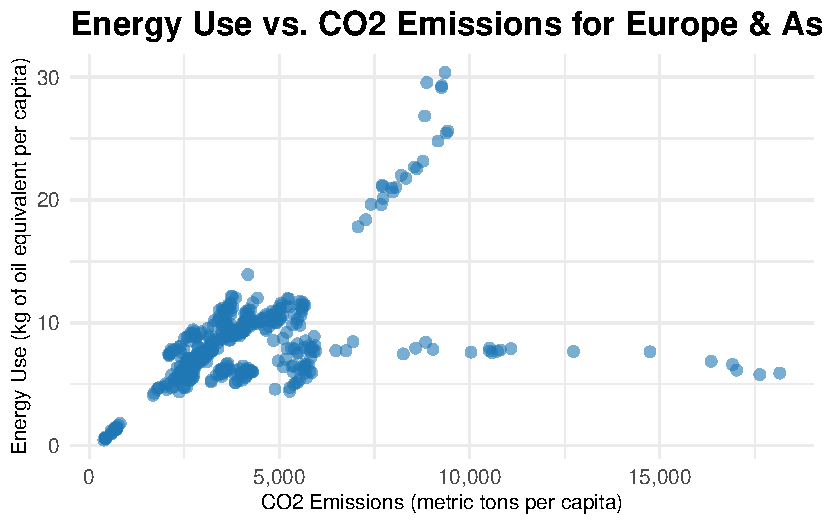
\includegraphics{Report_files/figure-pdf/unnamed-chunk-21-1.pdf}

\begin{itemize}
\tightlist
\item
  The majority of the population in the countries of Europe and Asia
  have concentrated energy use from 5 to 12.5 kg of oil equivalent per
  capita. The CO2 emission is equivalent to about 2500 to 7500 tons per
  capita.
\end{itemize}

\subsection{Urban Population vs CO2 Emissions}

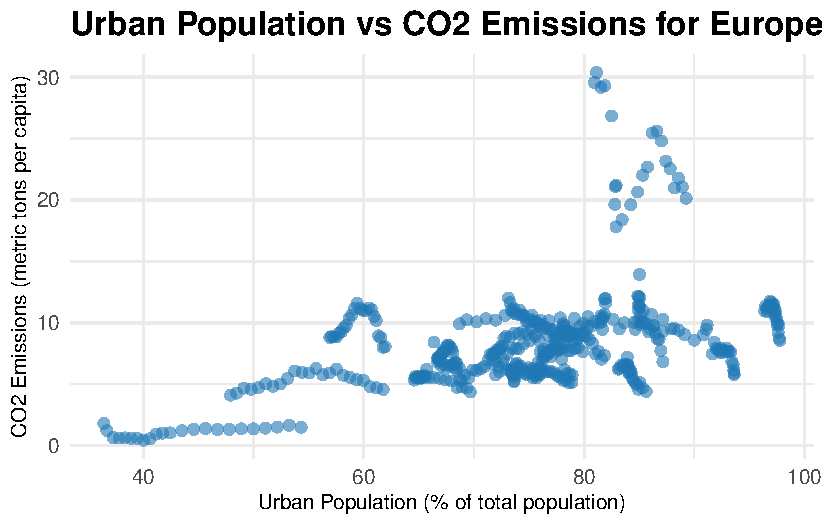
\includegraphics{Report_files/figure-pdf/unnamed-chunk-22-1.pdf}

\begin{itemize}
\tightlist
\item
  With the percentage of population in urban areas below 55\%, CO2
  consumption is quite low. Most cities have CO2 emissions of between 5
  and more than 10 tons per capita. There are also special situations
  where a few municipalities with a population distribution of 80 to
  90\% have extremely large CO2 emissions, about 20 to 30 tons per
  capita.
\end{itemize}

\subsection{Average GDP per Capita}

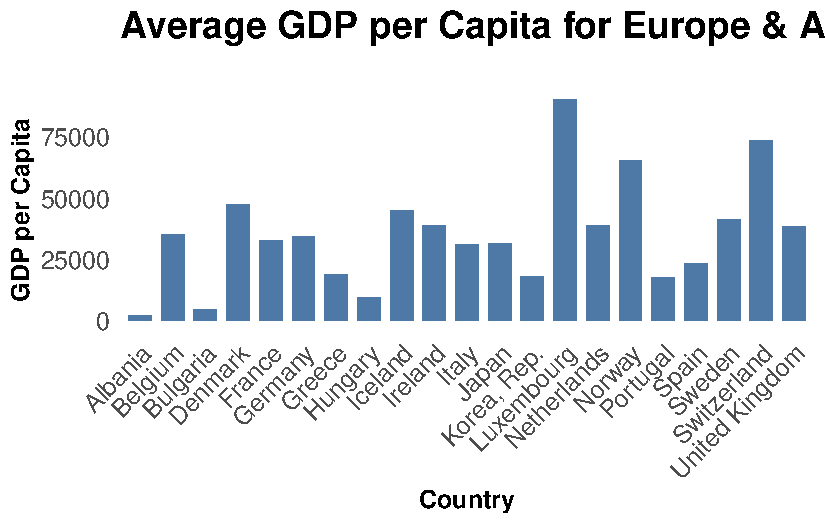
\includegraphics{Report_files/figure-pdf/unnamed-chunk-23-1.pdf}

\begin{center}\rule{0.5\linewidth}{0.5pt}\end{center}

\hypertarget{dynamic-panel-data-model-estimation}{%
\section{Dynamic Panel Data Model
Estimation}\label{dynamic-panel-data-model-estimation}}

\hypertarget{arellano-and-bond-1991-twostep-estimation-extended-by-nonlinear-moment-gmm}{%
\subsection{Arellano and Bond (1991) twostep estimation extended by
nonlinear moment
(GMM)}\label{arellano-and-bond-1991-twostep-estimation-extended-by-nonlinear-moment-gmm}}

The below hypothesis has been seek by research for e regions together
with global panel

\textbf{Hypothesis}:

if \(Y\) (GDP per capita) is positive and \(Y^2\) (Squared GDP per
capita) is negative we do have inverted U-shape pattern

The following tests should be satisfied for the Generalized Method of
Moments (GMM) estimation

\textbf{Sargan Test}:

\(H_o\): Overidentifying restrictions valid

In this context, we are looking for a p-value greater than 0.05.\\
For GMM estimation overidentifying restrictions have to be valid

\textbf{Autocorrelation test (2)}:

\(H_o\): no serial correlation of order 2 in epsilon

In this context, we are looking for a p-value greater than 0.05.\\
For GMM estimation we should not have second order serial correlation

\hypertarget{output-of-table-4-page-1107-in-the-article-result-for-the-global-panel}{%
\subsubsection{Output of Table 4 (page 1107 in the article) : Result for
the global
panel}\label{output-of-table-4-page-1107-in-the-article-result-for-the-global-panel}}

\begin{verbatim}
Twoways effects One-step model System GMM 

Call:
pgmm(formula = log(C) ~ lag(log(C), 1) + log(Y) + logY2 + log(E) + 
    log(URB) + log(TR) | lag(log(C), 0:20), data = dfglobalPanel, 
    effect = "twoways", model = "onestep", transformation = "ld")

Unbalanced Panel: n = 56, T = 2-23, N = 1252

Number of Observations Used: 2336
Residuals:
      Min.    1st Qu.     Median       Mean    3rd Qu.       Max. 
-0.8498393 -0.0441124  0.0010610  0.0000626  0.0448673  0.9416527 

Coefficients:
                 Estimate Std. Error z-value  Pr(>|z|)    
lag(log(C), 1)  0.9055286  0.0219538 41.2470 < 2.2e-16 ***
log(Y)          0.3183996  0.0798754  3.9862 6.714e-05 ***
logY2          -0.0170164  0.0043737 -3.8906 9.999e-05 ***
log(E)          0.0708023  0.0282166  2.5092   0.01210 *  
log(URB)        0.0552130  0.0281454  1.9617   0.04980 *  
log(TR)         0.0238843  0.0112268  2.1274   0.03338 *  
---
Signif. codes:  0 '***' 0.001 '**' 0.01 '*' 0.05 '.' 0.1 ' ' 1

Sargan test: chisq(295) = 54.53814 (p-value = 1)
Autocorrelation test (1): normal = -4.212125 (p-value = 2.5298e-05)
Autocorrelation test (2): normal = -0.9451604 (p-value = 0.34458)
Wald test for coefficients: chisq(6) = 43646.02 (p-value = < 2.22e-16)
Wald test for time dummies: chisq(21) = 73.13811 (p-value = 1.094e-07)
\end{verbatim}

\begin{itemize}
\item
  For the global panel the null hypothesis of no serial correlation
  (Autocorrelation test (2)) cannot be rejected, given the p-value
  \textgreater{} 0.05 and absence of a second order of correlation.
\item
  For the global panel the Sargan test statistics to assess the validity
  of overidentifying restrictions.The test yielded a p-value of 1, and
  thus we fail to reject the null hypothesis that the overidentifying
  restrictions are valid.
\item
  For the global panel The results of the \textbf{Sargan} test and
  \textbf{AR(2)} analysis are consistent with the author's findings.
\item
  In contrast to the author's findings of the global panel , our panel
  data model shows that all variables are statistically significant,
  including Trade.
\item
  Our model of the the global panel indicates a positive effect of
  lagged CO2 emissions on current CO2 emissions, whereas the author's
  findings of global panel showed a negative effect of lagged CO2
  emissions on current CO2 emissions.
\item
  Our model of the the global panel indicates a positive impact of urban
  population on CO2 emissions, whereas the author's findings of global
  panel showed a negative impact of urban population on CO2 emissions.
\item
  Our model of the the global panel indicates that the hypothesis is
  valid for the global panel due to \(log(Y)>0\text{ and }log(Y^2) <0\),
  However, the author's findings show that the hypothesis is invalid.
\end{itemize}

\hypertarget{output-of-table-56-page-1107-and-1108-in-the-article-european-and-north-asian-region-countries}{%
\subsubsection{Output of Table 5,6 (page 1107 and 1108 in the article) :
European and North Asian region
countries}\label{output-of-table-56-page-1107-and-1108-in-the-article-european-and-north-asian-region-countries}}

\begin{verbatim}
Twoways effects One-step model System GMM 

Call:
pgmm(formula = log(C) ~ lag(log(C), 1) + log(Y) + logY2 + log(E) + 
    log(URB) + log(TR) | lag(log(C), 0:20), data = dfEuropeAsia, 
    effect = "twoways", model = "onestep", transformation = "ld")

Unbalanced Panel: n = 21, T = 18-23, N = 477

Number of Observations Used: 891
Residuals:
      Min.    1st Qu.     Median       Mean    3rd Qu.       Max. 
-0.4139063 -0.0454911  0.0036730  0.0000039  0.0489629  0.3197112 

Coefficients:
                Estimate Std. Error z-value  Pr(>|z|)    
lag(log(C), 1)  0.629021   0.075995  8.2771 < 2.2e-16 ***
log(Y)          1.328676   0.323373  4.1088 3.977e-05 ***
logY2          -0.064168   0.016788 -3.8224 0.0001322 ***
log(E)          0.050945   0.108015  0.4717 0.6371764    
log(URB)        0.288537   0.132028  2.1854 0.0288584 *  
log(TR)         0.111616   0.059419  1.8785 0.0603172 .  
---
Signif. codes:  0 '***' 0.001 '**' 0.01 '*' 0.05 '.' 0.1 ' ' 1

Sargan test: chisq(295) = 21 (p-value = 1)
Autocorrelation test (1): normal = -2.872327 (p-value = 0.0040746)
Autocorrelation test (2): normal = -0.8128054 (p-value = 0.41633)
Wald test for coefficients: chisq(6) = 2174.835 (p-value = < 2.22e-16)
Wald test for time dummies: chisq(21) = -200733605 (p-value = 1)
\end{verbatim}

\begin{itemize}
\item
  For European and North Asian region countries the null hypothesis of
  no serial correlation (Autocorrelation test (2)) cannot be rejected,
  given the p-value \textgreater{} 0.05 and absence of a second order of
  correlation.
\item
  For European and North Asian region countries the Sargan test
  statistics to assess the validity of overidentifying restrictions.The
  test yielded a p-value of 1, and thus we fail to reject the null
  hypothesis that the overidentifying restrictions are valid.
\item
  For European and North Asian region countries the results of the
  \textbf{Sargan} test and \textbf{AR(2)} analysis are consistent with
  the author's findings.
\item
  For European and North Asian region countries While the author's
  findings suggest that only urban population is statistically
  insignificant, our model indicates that only energy use is
  statistically insignificant.
\item
  For European and North Asian region countries it appears that there is
  a discrepancy between the author's findings and our model. The
  author's findings indicate that urban population and trade have a
  negative impact on CO2 emissions, while our model indicates a positive
  impact.
\item
  Our findings indicate that the hypothesis is valid for the European
  and North Asian region countries, as we observed an inverted U-shape
  pattern, which is consistent with the author's findings.
\end{itemize}

\hypertarget{output-of-table-56-page-1107-and-1108-in-the-article-latin-american-and-caribbean-region-countries}{%
\subsubsection{Output of Table 5,6 (page 1107 and 1108 in the article) :
Latin American and Caribbean region
countries}\label{output-of-table-56-page-1107-and-1108-in-the-article-latin-american-and-caribbean-region-countries}}

\begin{verbatim}
Oneway (individual) effect One-step model System GMM 

Call:
pgmm(formula = log(C) ~ lag(log(C), 1) + log(Y) + logY2 + log(E) + 
    log(URB) + log(TR) | lag(log(C), 0:20), data = dfLACarrb, 
    effect = "individual", model = "onestep", transformation = "ld")

Balanced Panel: n = 14, T = 23, N = 322

Number of Observations Used: 602
Residuals:
      Min.    1st Qu.     Median       Mean    3rd Qu.       Max. 
-0.3245483 -0.0536620  0.0018657  0.0001758  0.0554823  0.3060322 

Coefficients:
                 Estimate Std. Error z-value  Pr(>|z|)    
lag(log(C), 1)  0.7007167  0.0434015 16.1450 < 2.2e-16 ***
log(Y)         -0.5750419  0.1500535 -3.8322  0.000127 ***
logY2           0.0373058  0.0078367  4.7604 1.932e-06 ***
log(E)          0.2098909  0.0812726  2.5826  0.009807 ** 
log(URB)        0.1953495  0.1423838  1.3720  0.170066    
log(TR)         0.0214684  0.0290549  0.7389  0.459973    
---
Signif. codes:  0 '***' 0.001 '**' 0.01 '*' 0.05 '.' 0.1 ' ' 1

Sargan test: chisq(295) = 14 (p-value = 1)
Autocorrelation test (1): normal = -3.13654 (p-value = 0.0017095)
Autocorrelation test (2): normal = 0.4197642 (p-value = 0.67466)
Wald test for coefficients: chisq(6) = 2455.748 (p-value = < 2.22e-16)
\end{verbatim}

\begin{itemize}
\item
  For Latin American and Caribbean region countries the null hypothesis
  of no serial correlation (Autocorrelation test (2)) cannot be
  rejected, given the p-value \textgreater{} 0.05 and absence of a
  second order of correlation.
\item
  For Latin American and Caribbean region countries the Sargan test
  statistics to assess the validity of overidentifying restrictions.The
  test yielded a p-value of 1, and thus we fail to reject the null
  hypothesis that the overidentifying restrictions are valid.
\item
  For Latin American and Caribbean region countries the results of the
  \textbf{Sargan} test and \textbf{AR(2)} analysis are consistent with
  the author's findings
\item
  Our model for Latin American and Caribbean region countries suggests
  that the lagged CO2 emissions variable is statistically significant,
  while it is not the case in the author's findings.
\item
  Our findings suggest that the hypothesis is invalid for the Latin
  American and Caribbean region countries,which is consistent with the
  author's findings.
\end{itemize}

\hypertarget{output-of-table-56-page-1107-and-1108-in-the-article-middle-eastern-north-african-and-sub-saharan-region-countries}{%
\subsubsection{Output of Table 5,6 (page 1107 and 1108 in the article) :
Middle Eastern, North African, and sub-Saharan region
countries}\label{output-of-table-56-page-1107-and-1108-in-the-article-middle-eastern-north-african-and-sub-saharan-region-countries}}

\begin{verbatim}
Twoways effects One-step model System GMM 

Call:
pgmm(formula = log(C) ~ lag(log(C), 1) + log(Y) + logY2 + log(E) + 
    log(URB) + log(TR) | lag(log(C), 0:20), data = dfMeNoAfrSub, 
    effect = "twoways", model = "onestep", transformation = "ld")

Unbalanced Panel: n = 21, T = 2-23, N = 453

Number of Observations Used: 843
Residuals:
      Min.    1st Qu.     Median       Mean    3rd Qu.       Max. 
-0.8480802 -0.0559806  0.0011687  0.0000767  0.0579469  0.8942252 

Coefficients:
                Estimate Std. Error z-value  Pr(>|z|)    
lag(log(C), 1)  0.833446   0.038147 21.8481 < 2.2e-16 ***
log(Y)          0.914166   0.328846  2.7799  0.005437 ** 
logY2          -0.056476   0.022911 -2.4650  0.013699 *  
log(E)          0.175736   0.071104  2.4716  0.013453 *  
log(URB)        0.178331   0.062901  2.8351  0.004581 ** 
log(TR)         0.050622   0.042228  1.1988  0.230613    
---
Signif. codes:  0 '***' 0.001 '**' 0.01 '*' 0.05 '.' 0.1 ' ' 1

Sargan test: chisq(295) = 21 (p-value = 1)
Autocorrelation test (1): normal = -2.318918 (p-value = 0.0204)
Autocorrelation test (2): normal = -0.4254173 (p-value = 0.67053)
Wald test for coefficients: chisq(6) = 10397.41 (p-value = < 2.22e-16)
Wald test for time dummies: chisq(21) = -25845698855 (p-value = 1)
\end{verbatim}

\begin{itemize}
\item
  For Middle Eastern, North African, and sub-Saharan region countries
  the null hypothesis of no serial correlation (Autocorrelation test
  (2)) cannot be rejected, given the p-value \textgreater{} 0.05 and
  absence of a second order of correlation.
\item
  For Middle Eastern, North African, and sub-Saharan region countries
  the Sargan test statistics to assess the validity of overidentifying
  restrictions.The test yielded a p-value of 1, and thus we fail to
  reject the null hypothesis that the overidentifying restrictions are
  valid.
\item
  For Middle Eastern, North African, and sub-Saharan region countries
  the results of the \textbf{Sargan} test and \textbf{AR(2)} analysis
  are consistent with the author's findings
\item
  In the Middle Eastern, North African, and sub-Saharan region, the
  author's findings suggest that only urban population is statistically
  insignificant, while our model indicates that only trade is
  statistically insignificant.
\item
  For Middle Eastern, North African, and sub-Saharan region Countries
  our model indicates a positive effect of lagged CO2 emissions on
  current CO2 emissions, whereas the author's findings showed a negative
  effect of lagged CO2 emissions on current CO2 emissions.
\item
  For Middle Eastern, North African, and sub-Saharan region countries
  our model indicates a positive effect of trade on CO2 emissions,
  whereas the author's findings showed a negative effect of trade on CO2
  emissions. Nevertheless trade is statistically insignificant in our
  model
\item
  Our findings suggest that the hypothesis is valid for the Middle
  Eastern, North African, and sub-Saharan regions,which is consistent
  with the author's findings.
\end{itemize}

\begin{center}\rule{0.5\linewidth}{0.5pt}\end{center}

\hypertarget{conclusion}{%
\section{CONCLUSION}\label{conclusion}}

\begin{itemize}
\item
  Our findings showed that energy use\texttt{log(E)} has a positive
  impact on carbon dioxide emissions for all the panels, which is in
  line with the authors' results
\item
  Our findings showed that GDP per capita \texttt{log(Y)} has a
  positive, statistically significant impact on carbon dioxide emissions
  for the Global Panel, European and North Asian, Middle Eastern, North
  African, and sub-Saharan African regions, except for the Latin
  American and Caribbean regions, which is in line with the authors'
  results
\end{itemize}

\textbf{Does the presence of an inverted U-shaped curve observed ?}

\begin{longtable}[]{@{}
  >{\raggedright\arraybackslash}p{(\columnwidth - 6\tabcolsep) * \real{0.3622}}
  >{\raggedright\arraybackslash}p{(\columnwidth - 6\tabcolsep) * \real{0.1811}}
  >{\raggedright\arraybackslash}p{(\columnwidth - 6\tabcolsep) * \real{0.1102}}
  >{\raggedright\arraybackslash}p{(\columnwidth - 6\tabcolsep) * \real{0.3465}}@{}}
\toprule\noalign{}
\begin{minipage}[b]{\linewidth}\raggedright
Region
\end{minipage} & \begin{minipage}[b]{\linewidth}\raggedright
The author's findings
\end{minipage} & \begin{minipage}[b]{\linewidth}\raggedright
Our Findings
\end{minipage} & \begin{minipage}[b]{\linewidth}\raggedright
Does it align with the author's findings ?
\end{minipage} \\
\midrule\noalign{}
\endhead
\bottomrule\noalign{}
\endlastfoot
Global Panel & Not Valid & Valid & No \\
Europe and North Asian & Valid & Valid & Yes \\
Latin American and Caribbean & Not Valid & Not Valid & Yes \\
Middle Eastern, North African and Sub-Sharan & Valid & Valid & Yes \\
\end{longtable}



\end{document}
